%\subsubsection*{Dinic's Algorithm (1970)}

Following the Ford-Fulkerson method and the Edmonds-Karp algorithm, Dinic's Algorithm provides a more efficient framework for solving the maximum flow problem in networks. Dinic's Algorithm was originally introduced by Israeli computer scientist Yefim (Chaim) Dinitz in 1970. While primarily designed for general graphs, Dinic's Algorithm can effectively solve the maximum matching problem in bipartite graphs by modeling the matching as a flow problem. \cite{dinitz1970algorithm}.

\paragraph{Algorithm Overview}

To apply Dinic's Algorithm to the bipartite matching problem, the bipartite graph $G=(U,V,E)$ is transformed into a flow network $G'=(V',E')$ following the procedure outlined in Section~3.6.2, where:
\begin{itemize}
    \item $V'$ is the new set of vertices containing original vertices in $U$ and $V$, plus a source $s$ and a sink $t$.
    \item $E'$ is the new set of edges in which, for every edge $(u,v) \in E$, $u \in U$ and $v \in V$ are connected with capacity 1.
\end{itemize}

The maximum flow in this transformed network corresponds to the maximum matching in the bipartite graph, where each flow unit represents an edge in the matching \cite{cormen2009introduction}.

\textbf{Dinic’s Algorithm} can be divided into three main phases:
\begin{enumerate}
    \item The algorithm begins by constructing a level graph $L$. A level graph is derived from the residual graph $G(f)$, which represents the current state of flow in the network. $L$ ensures only edges forming the shortest augmenting paths (refer to Section~2.1.11 for definition) are considered in subsequent steps. A level graph is constructed by performing Breadth-First Search (BFS) from the source to assign levels to vertices based on the distance from $s$.
    \begin{figure}[ht]
        \centering
        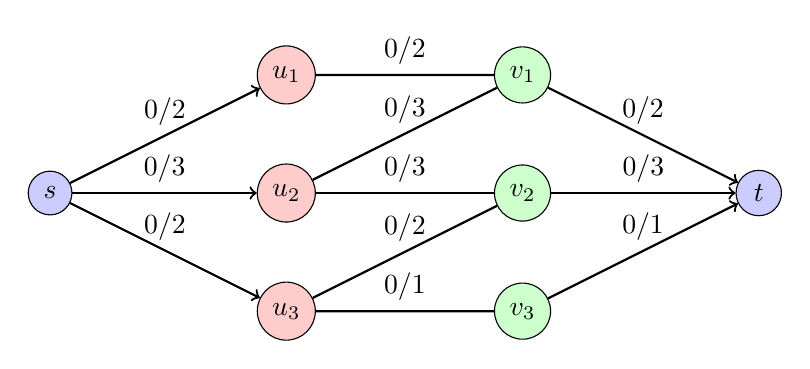
\begin{tikzpicture}[scale=1.5]
            % Draw nodes for source and sink
            \node[circle, draw, fill=blue!20] (s) at (-2, 0) {\(s\)};

            \node[circle, draw, fill=blue!20] (t) at (4, 0) {\(t\)};

        
            % Draw nodes for set U
            \node[circle, draw, fill=red!20] (u1) at (0, 1) {\(u_1\)};
            \node[circle, draw, fill=red!20] (u2) at (0, 0) {\(u_2\)};
            \node[circle, draw, fill=red!20] (u3) at (0, -1) {\(u_3\)};

        
            % Draw nodes for set V
            \node[circle, draw, fill=green!20] (v1) at (2, 1) {\(v_1\)};
            \node[circle, draw, fill=green!20] (v2) at (2, 0) {\(v_2\)};
            \node[circle, draw, fill=green!20] (v3) at (2, -1) {\(v_3\)};

        
            % Draw edges from source to set U
            \draw[thick, ->] (s) -- node[midway, above] {0/2} (u1);
            \draw[thick, ->] (s) -- node[midway, above] {0/3} (u2);
            \draw[thick, ->] (s) -- node[midway, above] {0/2} (u3);
            
        
            % Draw edges between U and V
            \draw[thick] (u1) -- node[midway, above] {0/2} (v1); % Edge between u1 and v1
            \draw[thick] (u2) -- node[midway, above] {0/3} (v1); % Edge between u2 and v1
            \draw[thick] (u2) -- node[midway, above] {0/3} (v2); % Edge between u2 and v2
            \draw[thick] (u3) -- node[midway, above] {0/2} (v2); % Edge between u3 and v2
            \draw[thick] (u3) -- node[midway, above] {0/1} (v3); % Edge between u3 and v3
        
            % Draw edges from set V to sink
            \draw[thick, ->] (v1) -- node[midway, above] {0/2} (t);
            \draw[thick, ->] (v2) -- node[midway, above] {0/3} (t);
            \draw[thick, ->] (v3) -- node[midway, above] {0/1} (t);
        
        \end{tikzpicture}
        \label{fig:level_graph}
        \caption{Initial graph \( G \) before BFS. All edges are shown with no level assignments.}
        \end{figure}
        

    \item Once the level graph \(L\) is constructed, the algorithm computes a \textit{blocking flow} in \(L\). A blocking flow is a flow such that no augmenting path from \(s\) to \(t\) exists within \(L\). This is achieved by identifying augmenting paths using Depth-First Search (DFS) and augmenting the flow along each path by the minimum residual capacity of the edges in the path. If an edge along a path is fully saturated (i.e., its residual capacity becomes zero), the path becomes invalid for further augmentation. By saturating at least one edge on every \(s \to t\) path, the algorithm ensures no further augmenting paths can exist in \(L\). After augmenting the flow, the residual capacities in the original graph \(G(f)\) are updated to reflect the changes. This process guarantees that the blocking flow fully utilizes the level graph for the current iteration before the next level graph is constructed.

    \begin{figure}[h]
        \centering
        \begin{tikzpicture}[scale=1.5]
            % Draw nodes for source and sink
            \node[circle, draw, fill=blue!20] (s) at (-2, 0) {\(s\)};
            \node[above=0.1cm of s] (L0) {\textbf{L0}};
            \node[circle, draw, fill=blue!20] (t) at (4, 0) {\(t\)};
            \node[above=0.1cm of t] (L3) {\textbf{L3}};
        
            % Draw nodes for set U
            \node[circle, draw, fill=red!20] (u1) at (0, 1) {\(u_1\)};
            \node[circle, draw, fill=red!20] (u2) at (0, 0) {\(u_2\)};
            \node[circle, draw, fill=red!20] (u3) at (0, -1) {\(u_3\)};

            \node[above=0.1cm of u1] (L1) {\textbf{L1}};
            \node[above=0.1cm of u2] (L1) {\textbf{L1}};
            \node[above=0.1cm of u3] (L1) {\textbf{L1}};
        
            % Draw nodes for set V
            \node[circle, draw, fill=green!20] (v1) at (2, 1) {\(v_1\)};
            \node[circle, draw, fill=green!20] (v2) at (2, 0) {\(v_2\)};
            \node[circle, draw, fill=green!20] (v3) at (2, -1) {\(v_3\)};
            \node[above=0.1cm of v1] (L2) {\textbf{L2}};
            \node[above=0.1cm of v2] (L2) {\textbf{L2}};
            \node[above=0.1cm of v3] (L2) {\textbf{L2}};
        
          % Draw edges from source to set U
          \draw[thick, ->] (s) -- node[midway, above] {0/2} (u1);
          \draw[thick, ->] (s) -- node[midway, above] {3/3} (u2);
          \draw[thick, ->] (s) -- node[midway, above] {2/2} (u3);
          
      
          % Draw edges between U and V
          \draw[thick] (u1) -- node[midway, above] {0/2} (v1); % Edge between u1 and v1
          \draw[thick] (u2) -- node[midway, above] {2/3} (v1); % Edge between u2 and v1
          \draw[thick] (u2) -- node[midway, above] {1/3} (v2); % Edge between u2 and v2
          \draw[thick] (u3) -- node[midway, above] {1/2} (v2); % Edge between u3 and v2
          \draw[thick] (u3) -- node[midway, above] {1/1} (v3); % Edge between u3 and v3
      
        % Draw edges from set V to sink
        \draw[thick, ->] (v1) -- node[midway, above] {2/2} (t);
        \draw[thick, ->] (v2) -- node[midway, above] {2/3} (t);
        \draw[thick, ->] (v3) -- node[midway, above] {1/1} (t);
        
        % Highlight shortest augmenting paths in BFS
        \draw[ultra thick, blue, ->] (s) -- (u2); % Shortest path to u2
        \draw[ultra thick, blue] (u2) -- (v1); % Shortest path from u2 to v1
        \draw[ultra thick, blue, ->] (v1) -- (t); % Shortest path to sink

        \draw[ultra thick, blue, ->] (s) -- (u3); % Shortest path to u2
        \draw[ultra thick, blue] (u3) -- (v3); % Shortest path from u2 to v1
        \draw[ultra thick, blue, ->] (v3) -- (t); % Shortest path to sink

        \draw[ultra thick, blue, ->] (s) -- (u2); % Shortest path to u2
        \draw[ultra thick, blue] (u2) -- (v2); % Shortest path from u2 to v1
        \draw[ultra thick, blue, ->] (v2) -- (t); % Shortest path to sink
        
        \draw[ultra thick, blue, ->] (s) -- (u3); % Shortest path to u2
        \draw[ultra thick, blue] (u3) -- (v2); % Shortest path from u2 to v1
        \draw[ultra thick, blue, ->] (v2) -- (t); % Shortest path to sink
        
        \end{tikzpicture}
        
        \label{fig:level_graph}
        \caption{Construction of the level graph \( L \) in Dinic's Algorithm, illustrating the level graph after performing BFS.}
        \end{figure}

\paragraph{}Figures above illustrate the process of constructing a level graph \( L \) from the initial graph \( G \) in Dinic's Algorithm. Figure 3.1 shows the initial graph \( G \), which represents the network before performing any operations. In this state, all edges and vertices are present, but no levels are assigned to the nodes. Figure 3.2 represents the level graph \( L \) after applying a Breadth-First Search (BFS) on the residual graph \( G(f) \). BFS begins from the source node \( s \) and assigns levels to vertices based on their shortest distance from \( s \). These levels, denoted as \( L0, L1, L2, \) and \( L3 \), correspond to increasing distances from the source. In the example, BFS finds a shortest augmenting path \( s \to u_2 \to v_1 \to t \), which is highlighted in blue. For the path \( s \to u_2 \to v_1 \to t \), maximum amount of flow that can be pushed along this path is $\min\{ c_f(s, u_2), c_f(u_2, v_1), c_f(v_1, t) \} = 2$. After that, it is added to the flow along each edge in the augmenting path, and we update the residual capacities. Notice how we are sending four flows together. This is where it is optimized compared to Edmond Karp where we send one flow at a time. 
\begin{itemize}
    \item 2 units of flow on path \( s \to u_2 \to v_1 \to t \)
    \item 1 unit of flow on path \( s \to u_3 \to v_3 \to t \)
    \item 1 unit of flow on path \( s \to u_3 \to v_2 \to t \)
    \item 1 unit of flow on path \( s \to u_2 \to v_2 \to t \)
    \item Total flow is:5
\end{itemize}

    
    \paragraph{} Now, since we achieve the first blocking flow iteration, we repeat the process by rebuilding the level graph. This time it should look different because the remaining capacities of multiple edges have changed.

    \begin{figure}[h]
        \centering
        \begin{tikzpicture}[scale=1.5]
            % Draw nodes for source and sink
            \node[circle, draw, fill=blue!20] (s) at (-2, 0) {\(s\)};
            \node[above=0.1cm of s] (L0) {\textbf{L0}};
            \node[circle, draw, fill=blue!20] (t) at (4, 0) {\(t\)};
            \node[above=0.1cm of t] (L3) {\textbf{L5}};
        
            % Draw nodes for set U
            \node[circle, draw, fill=red!20] (u1) at (0, 1) {\(u_1\)};
            \node[circle, draw, fill=red!20] (u2) at (0, 0) {\(u_2\)};
            \node[circle, draw, fill=red!20] (u3) at (0, -1) {\(u_3\)};

            \node[above=0.1cm of u1] (L1) {\textbf{L1}};
            \node[above=0.1cm of u2] (L3) {\textbf{L3}};
        
            % Draw nodes for set V
            \node[circle, draw, fill=green!20] (v1) at (2, 1) {\(v_1\)};
            \node[circle, draw, fill=green!20] (v2) at (2, 0) {\(v_2\)};
            \node[circle, draw, fill=green!20] (v3) at (2, -1) {\(v_3\)};
            \node[above=0.1cm of v1] (L2) {\textbf{L2}};
            \node[above=0.1cm of v2] (L2) {\textbf{L4}};
        
          % Draw edges from source to set U
          \draw[thick, ->] (s) -- node[midway, above] {1/2} (u1);
          \draw[thick, ->] (s) -- node[midway, above] {3/3} (u2);
          \draw[thick, ->] (s) -- node[midway, above] {2/2} (u3);
          
      
          % Draw edges between U and V
          \draw[thick] (u1) -- node[midway, above] {1/2} (v1); % Edge between u1 and v1
          \draw[thick] (u2) -- node[midway, above] {2/3} (v1); % Edge between u2 and v1
          \draw[thick] (u2) -- node[midway, above] {1/3} (v2); % Edge between u2 and v2
          \draw[thick] (u3) -- node[midway, above] {1/2} (v2); % Edge between u3 and v2
          \draw[thick] (u3) -- node[midway, above] {1/1} (v3); % Edge between u3 and v3
      
        % Draw edges from set V to sink
        \draw[thick, ->] (v1) -- node[midway, above] {2/2} (t);
        \draw[thick, ->] (v2) -- node[midway, above] {3/3} (t);
        \draw[thick, ->] (v3) -- node[midway, above] {1/1} (t);
        
        % Highlight shortest augmenting paths in BFS
        \draw[ultra thick, blue, ->] (s) -- (u1); % Shortest path to u2
        \draw[ultra thick, blue] (u1) -- (v1); % Shortest path from u2 to v1
        \draw[ultra thick, blue, ->] (v1) -- (u2); % Shortest path to sink
        \draw[ultra thick, blue, ->] (u2) -- (v2); % Shortest path to sink
        \draw[ultra thick, blue, ->] (v2) -- (t); % Shortest path to sink
        \end{tikzpicture}
        
        \label{fig:level_graph}
        \caption{Construction of the level graph \( L \) in Dinic's Algorithm, illustrating the level graph after performing BFS.}
        \end{figure}
    
    \paragraph{} After this phase:
    \begin{itemize}
        \item 1 unit of flow on path \( s \to u_1 \to v_1 \to u2 \to v2 \to t \)
        \item Total flow is: 5 + 1 = 6
    \end{itemize}

    \paragraph{} Here, a block flow is achieved, and there are no more flows can be pushed through the network. Program terminates.

                    
    \item The algorithm iterates between constructing a level graph and computing a blocking flow until no augmenting paths can be found, at which point the maximum flow (and thus the maximum matching) has been achieved.
\end{enumerate}

\paragraph{Pseudocode}
In the context of bipartite maximum matching, the input is a bipartite graph $G = (U, V, E)$, where $U$ and $V$ are two disjoint sets of vertices, and $E$ is the set of edges connecting them. As stated above, the problem is converted into a network flow: $G =((V,E),c,f,s,t)$. Dinic's Algorithm proceeds as follows:

\begin{algorithm}
    \caption{Dinic's Algorithm for Maximum Bipartite Matching}
    
    \textbf{Input:} A network \( G = ((V, E), c, s, t) \). \\
    \textbf{Output:} An \( s \)–\( t \) flow \( f \) of maximum value.
    
    \begin{algorithmic}[1]
    \STATE Initialize \( f(e) \gets 0 \) for each \( e \in E \).
    \WHILE{true}
        \STATE Construct the level graph \( G_L \) from the residual graph \( G(f) \) using BFS.
        \IF{\( \text{dist}(t) = \infty \)}
            \STATE \textbf{break} (No more augmenting paths exist).
        \ENDIF
        \WHILE{A blocking flow \( f' \) can be found in \( G_L \)}
            \STATE Augment the flow \( f \) by \( f' \).
            \STATE Update the residual capacities in \( G(f) \).
        \ENDWHILE
    \ENDWHILE
    \RETURN \( f \)
    \end{algorithmic}
    \end{algorithm}    

\paragraph{Explanation}

Going line by line:
\begin{itemize}
    \item \textbf{Line 1:} Initializes all flows $f(e)$ to zero for each edge $e \in E$.
    \item \textbf{Line 2-5:} A breadth-first search (BFS) is performed on the residual graph $G(f)$ to compute the shortest path distances $\text{dist}(v)$ from the source $s$ to every vertex $v$. Using these distances, the level graph $G(L)$ is built. This graph only includes edges $(u,v) \in E(f)$ that satisfy $\text{dist}(v)=\text{dist}(u)+1$. If $\text{dist}(t)=\infty$, no $s$-$t$ path exists, and the algorithm terminates, confirming that the current flow is the maximum flow.
    \item \textbf{Line 6:} A blocking flow $f'$ is computed within $G(L)$. This is a flow where every $s$-$t$ path in $G(L)$ has at least one saturated edge (i.e., flow equals capacity).
    \item \textbf{Line 7-8:} By definition, $f'$ ensures no further flow can be sent along any $s$-$t$ path in $G(L)$, completing the current iteration of the algorithm.
    \item \textbf{Line 9:} Return the maximum flow.
\end{itemize}

\paragraph{Performance and Time Complexity}

The level graph $G(L)$ is built using a breadth-first search (BFS) on the residual graph $G(f)$. BFS runs in $O(V + E)$ time, where $V$ is the number of vertices and $E$ is the number of edges. To find a blocking flow, the most common method is to use a depth-first search (DFS) approach. Each edge in $G(L)$ is traversed at most once during a single computation of $f'$, making the blocking flow computation run in $O(E)$. Augmenting the flow also takes $O(E)$ time.

In bipartite maximum matching problems, all edges have unit capacity. The residual graph's depth (or the number of levels in $G(L)$) is limited by the number of edges in the longest augmenting path. This depth is proportional to $O(\sqrt{V})$, as the level graph represents alternating layers of vertices in the bipartite structure. Hence, at most $O(\sqrt{V})$ level graphs are needed for the entire algorithm. This explains the $O(\sqrt{V} \cdot E)$ performance for bipartite graphs, where the algorithm iteratively builds and uses $O(\sqrt{V})$ level graphs, each requiring $O(E)$ work.

\paragraph{Applications and Limitations}

Dinic’s Algorithm has applications in diverse fields such as network optimization, scheduling, and resource allocation. It is particularly effective in bipartite matching problems, with uses in image segmentation, community detection, and compiler optimizations. However, it is less efficient for dense graphs due to $O(V^3)$ complexity when $E = O(V^2)$, reflecting the worst-case complexity in fully connected networks. $O(\sqrt{V} \cdot E)$ applies to sparse bipartite graphs, while the $O(V^3)$ upper bound applies in dense graph scenarios.

